%!TEX root=../document.tex

\section{Grundlagen}
\label{sec:grundlagen}

\subsection{Qubit}
\label{sec:qubit}

\subsubsection{Schrödinger}
\label{sec:schrodinger}

Schroedingers Katze ist die berühmteste Veranschaulichung eines grundlegenden Phänomens der Quantenmechanik. Genaugenommen ist es ein Versuchsaufbau, anhand dessen sich verschiedene Begriffe der Quantenmechanik leicht erklären lassen. Der Versuchsaufbau sieht folgendermaßen aus:

In einer Kiste befinden sich eine Katze und eine Ampulle mit einer Giftigen Substanz. Mit einer exakten Wahrscheinlichkeit von 50\% ist die Ampulle offen und die Katze bereits tot, mit einer genau gleich großen Wahrscheinlichkeit ist aber die Ampulle immer noch verschlossen und die Katze am Leben. Da wir nur die Außenseite der Kiste sehen und sie Schall und Geruchdicht ist, können wir nicht genau sagen, in welchem Zustand die Katze sich befindet. Es könnte also behauptet werden, dass sie gleichzeitig tot und lebendig ist.
Den Umstand, dass 2 (oft gegensätzliche) Zustände wahr sind, wird in der Quantenmechanik als Superposition bezeichnet. Eine Vorraussetzung für das erreichen einer Superposition ist die vollkommene Abschottung von der Außenwelt. 

Wenn nun die Kiste geöffnet wird und der Betrachter einen Blick ins innere der Kiste wirft, so erkennt er ziemlich schnell, ob die Katze tot oder lebendig ist. Einer der Beiden Zustände ist durch diese sogenannte Messung verloren gegangen.

\subsubsection{Definition}
\label{sec:bit_definition}

Per Definition werden die Zustände eines Quantenbits in der Form $\alpha * |0\rangle + \beta * |1\rangle$ angeschrieben.
$\alpha$ und $\beta$ werden ''Amplituden'' genannt, sind komplexe Zahlen, stellen einen Anteil am Gesamtzustand dar und sind durch die Formel $|\alpha|^2 + |\beta|^2 = 1$ voneinander abhängig.

Dank der folgenden Umrechnung kann ein Qubit auch als Vektor geschrieben werden.

$\alpha|0\rangle+\beta|1\rangle = \alpha(1\choose0)+\beta(0\choose1) = (\alpha \choose \beta)$

\begin{figure}[!htb]
	\centering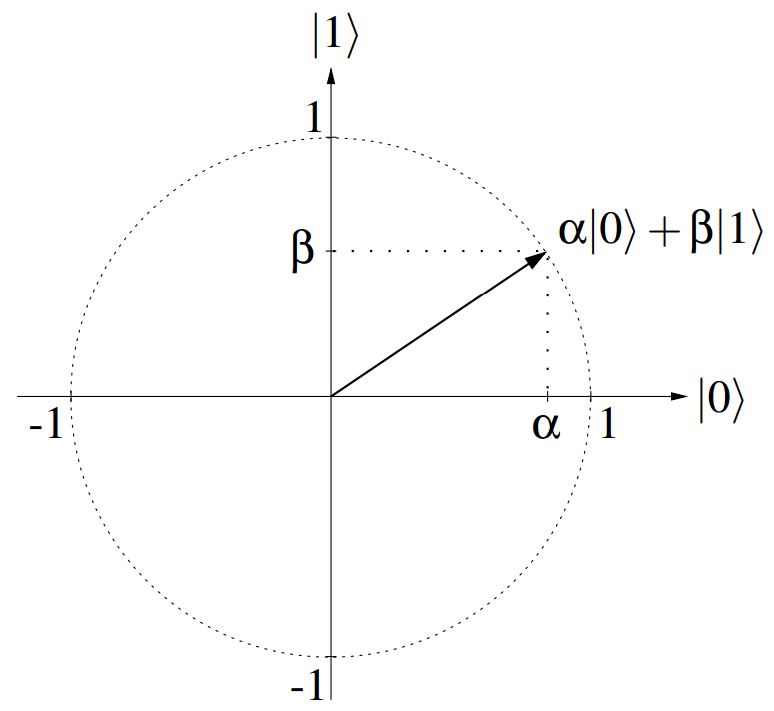
\includegraphics[width=0.8\textwidth]{images/vektor.jpg}
	\caption{Die Superposition als Vektor}
	\label{vektor}
\end{figure}

\subsubsection{Messung}
\label{sec:bit_messung}

Anders als ein klassisches Bit, kann ein Qubit nicht gelesen, sondern muss gemessen werden, wobei die Superposition zerstört wird.

Die Messung erfolgt je nach Ausführung des Quantenbits, da es auf mehrere Arten realisiert werden kann. Wenn Licht eine Rolle spielt, kann die Lichtstärke gemessen werden, wobei diese Art von Qubits nur kürzer als 1 Minuten gespeichert werden kann. Kernspinquantenbits können durch Messung der Magnetfelder, Ionenfallen mithilfe eines Lasers ausgelesen werden. Mehr dazu befindet sich im Kapitel Architektur.

\subsubsection{Zustände}
\label{sec:zustaende}

Bei der Messung eines Quantenbits im Zustand $\alpha|0\rangle+\beta|1\rangle$ wird die Superposition zerstört, wodurch das Quantenbit mit der Wahrscheinlichkeit $|\alpha|^2$ den Zustand $|0\rangle$ und mit der Wahrscheinlichkeit $|\beta|^2$ den Zustand $|1\rangle$ annimmt.

\subsubsection{Verschränkung}
\label{sec:verschraenkung}

2 Verschränkte Qubits haben die besondere Eigenschaften, dass sie sich unabhäng von der Distanz im genau gleichen Zustand befinden. Bei der Messung des einen Qubits wird die Superpositon beider Qubits zerstört und sie nehmen den selben wert an, der dann auch beim anderen Qubit gemessen werden kann.

\subsubsection{(De)Kohärenz}
\label{sec:koharenz}

Kohärenz bedeutet Zusammenhängend. Dekohärenz ist ein Phänomen der Quantenphysik, das Kohärenzeigenschaften von Systemen kurzzeitig außer Kraft setzt. Dekohärenzeffekte treten auf, wenn ein geschlossenes System geöffnet wird und mit der Umwelt in Wechselwirkung treten kann, wobei die Zustände beider Systeme irreversibel verändert werden.
Im Beispiel mit der Katze, wäre es eine Tote oder lebende Katze, und der Betrachter, der nun weiß, ob die Katze tot oder lebendig ist.

\subsection{Register}
\label{sec:register}

\subsubsection{Definition}
\label{sec:register_definition}
(formeln auf seite 28)

Ein Quantenregister besteht aus einer Reihe von 2 bis n Qubits und wird angeschrieben als $R = |x_1\ranlge|x_0\rangle$
Zur Erklärung ist allerdings eine Beschränkung auf das Minumum von 2 Bits sinnvoll.

\subsubsection{Berechnung}
\label{sec:register_berechnung}

Die Berechnung des Zustands eines Quantenregisters mit 2 Bit sieht folgendermaßen aus:
\begin{itemize}
    \item $|x_0\ranlge = \gamma|0\rangle + \gamma_1\rangle, |x_1\ranlge = \beta|0\rangle + \beta|1\rangle$
    \item $R = |x_1\ranlge|x_0\rangle$
	\item[=] $(\beta_0|0\rangle+\beta_1|1\rangle)(\gamma_0|0\rangle+\gamma_1|1\rangle)$
	\item[=] $\beta_0\gamma_0|0\rangle|0\rangle+\beta_0\gamma_1|0\rangle|1\rangle+\beta_1\gamma_0|1\rangle|0\rangle+\beta_1\gamma_1|1\rangle|1\rangle$
\end{itemize}

Zur Übersichtlichkeit wird angenommen, das
\begin{itemize}
	\item $\alpha_{i,j} = \beta_i\gamma_j$ und
	\item $|x_1\rangle|x_0\rangle = |x_1 x_0\rangle$
\end{itemize}
sowie die Ziffern vom binären ins dezimale Zahlensystem umgerechnet, wodurch folgende Schreibweise zustande kommt:

$R = \alpha_0|0\rangle+\alpha_1|1\rangle+\alpha_2|2\rangle+\alpha_3|3\rangle$

\subsubsection{Zustände}
\label{sec:zustande}

per Definition kann sich ein Quantenregister in Zuständen der Form

$R = \displaystyle\sum_{i=0}^{2^n-1} \alpha_1|i\rangle$

befinden, wobei die Einschränkung der einzelnen Qubits nicht vergessen werden darf, die für ein Register auf folgende Art erweitert werden kann:

$\displaystyle\sum_{i=0}^{2^n-1}  |\alpha|^2 = 1$

\subsubsection{Begriffe ''lokal'' und ''unitär''}
\label{sec:lokal_unitar}

Unitär bedeutet soviel wie Umkehrbar. Eine uniätre Operation kann also rückgängig gemacht werden. Die Voraussetzung dafür ist, dass es nur eine möglichkeit gibt, auf den Endzustand der Operation zu kommen. Wenn ein Endzustand von 2 verschiedenen Anfangszuständen erreicht werden kann, so ist nicht eindeutig, welcher Zustand der Anfangszustand ist und die Operation ist nicht unitär.

Rechenoperationen können auf einzelne Bits oder ganze Register ausgeführt werden. Da allerdings eine Rechenoperation auf ein ganzes Register auszuführen sehr schnell ziemlich kompliziert werden kann, führt man die Operation auf jedes Bit einzeln aus, wobei man das gleiche Gesamtergebnis erhält. Lokal ist eine Registertransformation, wenn daran für jede Operation konstant viele Qubits beteiligt sind.

\section{Hardware}
\label{sec:hardware}

\subsection{Gatter \& Transformationen}
\label{sec:gatter}

\subsubsection{Hadamard-Transformation}
\label{sec:hadamard}

Definiert ist die Hadamard-Transformation als Matrix $H = 1/\sqrt{2}\begin{pmatrix}1&1\\1&-1\end{pmatrix} $

Um die Hadamard-Matrix verwenden zu Können, muss das Qubit mithilfe der unitären Matrix $A = \begin{pmatrix}a&b\\c&d\end{pmatrix}$ folgendermaßen umgerechnet werden: $(\alpha'\choose\beta') = A(\alpha\choose\beta) = ({a\alpha + b\beta}\choose{c\alpha + d\beta})$

\subsubsection{CNOT}
\label{sec:cnot}

CNOT bedeutet ausgesprochen ''Controlled Not'', was als ''Kontrollierbare Negierungsschaltung'' übersetzt werden kann.
Ein CNOT hat 2 Eingänge und 2 Ausgänge, wobei der zweite Ausgang den invertierten Wert von 1 ausgibt wird, wenn der erste Eingang auf 1 gesetzt ist.

\begin{figure}[!htb]
	\centering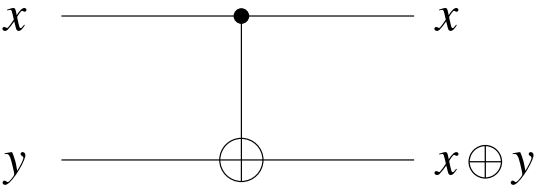
\includegraphics[width=0.8\textwidth]{images/cnot.jpg}
	\caption{CNOT-Gatter}
	\label{cnot}
\end{figure}

\subsection{Architektur}
\label{sec:architektur}

\subsubsection{Anforderungen}
\label{sec:anforderungen}

Definition von David Deutsch 1985:
Ein Quantencomputer besteht aus einer Reihe von Quantenbits,
\begin{enumerate}
	\item die in einen Anfangszustand versetzt werden können,
	\item die Information robust speichern,
	\item auf die (universelle) Quantengatter anwendbar sind und
	\item die gemessen werden können.
\end{enumerate}

\subsubsection{Photonen}
\label{sec:photonen}

Die Physiker Ludwig Mach und Ludwig Zehnder entwickelten unabhängig voneinander beide den selben Versuchsaufbau, der heutzutage Mach-Zender-Inferometer genannt wird. Er besteht aus 4 Spiegeln, wovon 2 halbdurchlässig sind, 2 Messgeräten und einem Streifen Papier.

Wenn ein Lichtstrahl in den Aufbau geschickt wird, so wird er über den ersten Spiegel, der halbdurchlässig ist, geteilt in eine gerade und eine um 90° abgelenkte Bahn gelenkt. Nach einem gewissen Abstand befindet sich auf jeder Bahn einer der "normalen" Spiegel, wodurch das Licht jeweils um 90° gelenkt wird und sich die beiden dann an einer Stelle kreuzen, an der der zweite halbdurchlässige Spiegel montiert wird. In eine Bahn wird ein Blatt Papier gehalten. Durch den halbdurchlässigen Spiegel kommt bei beiden Messgeräten gleich viel Licht an. Wird das Blatt Papier entfernt, so kommt es auf einer Bahn zu konstruktiven überlagerungen zwischen dem letzten Spiegel und dem Messgerät, wodurch bei diesem kein Licht ankommt.

Wenn anstelle eines Lichtstrahles nur einzelne Photonen verwendet werden, zeigt sich der selbe Effekt, obwohl eigentlich keines der Photonen wissen kann, ob der Papierstreifen im Weg ist oder nicht. Und hier kommt wieder die Quantenphysik als Erklärung zum einsatz, da ein Teilchen, wie wir schon wissen, solange es nicht beobachtet wird, in mehreren Zuständen gleichzeitig sein kann. Es kann sich also auf beiden Bahnen gleichzeitig bewegen, bis es gemessen wird, wodurch die Superposition zerstört wird und es nur bei einem Messgerät ankommen kann.

\subsubsection{Kernspinresonanz}
\label{sec:kernspinresonanz}

Kernspinresonanz ist der Name für einen phyiskalischen Effekt der in Form von Wechselwirkung zwischen Atomkernen und Magnetfeldern auftritt. Der Spin eines Moleküls kann durch Magnetfelder ausgerichtet werden, was ausgenutzt wird, um Quantenbits abzubilden und zu speichern. Durch unterschiedliche chemische Eigenschaften der Umgebung kann jedes Bit einzeln angesprochen werden. Mithilfe eines Hauptmagnetfeldes kann man die Zustande definieren, zum Beispiel als: $gleiche Ausrichtung = |0\rangle, im rechten Winkel = |1\rangle$;

\subsubsection{Ionenfallen}
\label{sec:ionenfallen}

Ionenfallen sind dazu da, um elektrisch geladene Moleküle oder Atome durch Magnetfelder an ein und der selben Position zu halten, wodurch mit einem gefangenen Ion bis zu 2 Quantenbits abgebildet werden können. Die abstände zwischen mehreren Ionen liegen im Mikrometerbereich, können durch einen Laser einzeln adressiert werden, aber müssen Temperaturmäßig nahe dem Absoluten gehalten werden um sich nicht gegenseitig abzustoßen.

\subsection{Umsetzung}
\label{sec:umsetzung}

\subsubsection{D-Wave Systems}
\label{sec:dwave}

D-Wave Systems ist ein 1999 gegründetes Amerikanischen Unternehmen, dass seit Jahren damit wirbt, den ersten und einzig wahren Quantencomputer herzustellen. D-Wave hat bereits Geräte an Lockhead-Martin, Google, NASA und die Kalifornische Universität verkauft.

Kritiker sind der Meinung, dass ein echter Quantencomputer erst in vielen Jahren möglich sein wird, falls überhaupt. Ein Google Test 2014 hat ergeben, dass keine Geschwindigkeitsveresserung festgestellt werden konnte. Anfang Dezember 2015 scheint durch eine weitere Google-Testreihe allerdings das Gegenteil bewiesen worden zu sein. In einem Test mit großen Bitmengen wurden laut Google Entwicklungsleiter Hartmut Neven eine Reihe herkömmlicher Großrechner zeitmäßig um Längen übertrumpft.

%https://www.wired.de/collection/latest/der-quantencomputer-d-wave-scheint-zu-funktionieren
%http://venturebeat.com/2015/12/08/google-says-its-quantum-computer-is-more-than-100-million-times-faster-than-a-regular-computer-chip/

Eine Forschungsarbeit an der ETH Zürich hat ergeben, dass der Quantencomputer eine Ein-Zweck-Maschine ist, für die ein Problem erst in ein passendes Format, bestehend aus einer großen Anzahl Variablen, gebracht werden muss, damit sie dann in relativ kurzer Zeit ein Optimum ermitteln kann. Sie hat aber weder etwas mit richtigen Quantenrechnern noch mit herkömmlichen Allzweckcomputern zu tun.

%http://www.spektrum.de/news/daempfer-fuer-den-d-wave-quantencomputer/1296152
%http://motherboard.vice.com/read/google-claims-its-d-wave-quantum-computer-is-the-real-deal

Die Arbeitsweise wird auf der offiziellen Webseite von D-Wave erklärt, wobei die Optimierung durch ''quantum annealing'' (direkt übersetzt: Quanten glühen) als die einzige art des Quantencomputing dargestellt wird.

%http://www.dwavesys.com/quantum-computing

Desweiteren findet man auf der offiziellen Webseite eine auflistung von Anwendungsgebieten, wobei die meisten auch als Mustererkennung und Vorraussagen bezeichnet werden könnten.

%http://www.dwavesys.com/quantum-computing/industries





%TODO bilder, gegenueberstellung,





\section{Interkommunikation}
\label{sec:interkommunikation}

\subsection{Quantennetzwerke/Kanäle}
\label{sec:Quantennetzwerke/Kanale}

\subsubsection{Klassische vs. Quanten-Kommunikationskanäle}
\label{sec:klassich_vs_quanten}

Zu den klassischen Kommunikationskanälen gehören eindeutig Kabel mit 1-n elektrisch Leitenden drähten, über die durch an- und ausschalten einzelne Bits übertragen werden können. Dieser Kommunikationsweg muss nach einer gewissen maximalen Strecke verstärkt werden, was zu verzögerungen führt.

Heutzutage zu klassichen Kommunikationskanälen, aber auch für die Übertragung von Qubits verwendbar, sind Glasfaserkabel. Im Klassischen Sinne wird Licht an und aus-geschalten, für Quantenkommunikation werden einzelne Qubits in form von Photonen übertragen.

Wenn man von Quantenkommunikationskanälen spricht, wird aber meist Verschränkung zwischen 2 Qubits gemeint. Dabei wird unterschieden zwischen rauschfreien und verrauschten Kanälen unterscheiden, wobei durch mehrfache Übertragungen mit klassischer Zusatzinformation aus einem verrauschten Kanal Stück für Stück ein rauschfreier Kanal machen lässt.

\subsubsection{Photonzählung}
\label{sec:photonzaelung}

Bei der Photonzälung werden zwischen 2 Standorten mit Sichtkontakt einzelne Photonen vom Sender ausgeschickt und vom Empfänger gezählt. Falls kein direkter Sichtkontakt besteht, können die Übertragungen auch über Glasfaserkabel erfolgen.

Praktisch getestet wurde es von Harald Weinfurter im Jahr 2007 mit einer Strecke von 144 km, wofür große Teleskope verwendet werden mussten.

\subsection{Quantenteleportation}
\label{sec:quantenteleportation}

Bei der Quantenteleportation sind 2 Qubits in form von Atomen an verschiedenen Orten durch Verschränkung verbunden. Bei einer Messung des Bits auf der ''Sender''-Seite wird die Superposition zerstört und beide Qubits nehmen zeitgleich den gleichen Zustand an. Da der Empfänger aber nicht wissen kann, wann der Sender das Bit betrachtet hat, muss über einen herkömmlichen Kanal ein Signal gesendet werden, dass den Empfänger imformiert, dass er sich das Qubit gefahrlos ansehen kann, ohne den Zustand zu verändern. Der zweite Grund für die Notwendigkeit der Übertragung eines Herkömmlichen Bits ist der, dass das Qubit beim Empfänger entweder durch Vertauschung mithilfe der Matrix $$ oder Transformation mithilfe der Matrix $$ gemappt werden muss.

Um allerdings 2 verschränkte Qubits an verschiedene Orte zu bringen, muss entwedet ein Quantenkanal bestehen oder schon im Vorfeld eines der verschränkten Qubits vom Sender zum Empfänger oder vom Empfänger zum Sender gebracht werden.

Da die Übertragung des herkömmlichen Bits nicht zeitgleich möglich ist, stellt sich die Frage, in welcher Form eine Quantenteleportation dann schneller ist. Die Antwort hängt mit Quantenregistern zusammen, da auch für ein komplettes Register nur ein einziges herkömmliches Bit übertragen werden muss.

